\documentclass[a4paper, 14pt]{extarticle}

% Поля
%--------------------------------------
\usepackage{geometry}
\geometry{a4paper,tmargin=2cm,bmargin=2cm,lmargin=3cm,rmargin=1cm}
%--------------------------------------


%Russian-specific packages
%--------------------------------------
\usepackage[T2A]{fontenc}
\usepackage[utf8]{inputenc}
\usepackage[english, main=russian]{babel}
\usepackage{cmap}
%--------------------------------------

\usepackage{textcomp}
\usepackage{amssymb}

% Красная строка
%--------------------------------------
\usepackage{indentfirst}               
%--------------------------------------             


%Graphics
%--------------------------------------
\usepackage{graphicx}
\graphicspath{ {./images/} }
\usepackage{wrapfig}
%--------------------------------------

% Полуторный интервал
%--------------------------------------
\linespread{1.3}                    
%--------------------------------------

%Выравнивание и переносы
%--------------------------------------
% Избавляемся от переполнений
\sloppy
% Запрещаем разрыв страницы после первой строки абзаца
\clubpenalty=10000
% Запрещаем разрыв страницы после последней строки абзаца
\widowpenalty=10000
%--------------------------------------

%Списки
\usepackage{enumitem}

%Подписи
\usepackage{caption} 

%Гиперссылки
\usepackage{hyperref}

\hypersetup {
	unicode=true
}

%Рисунки
%--------------------------------------
\DeclareCaptionLabelSeparator*{emdash}{~--- }
\captionsetup[figure]{labelsep=emdash,font=onehalfspacing,position=bottom}
%--------------------------------------

\usepackage{tempora}
\usepackage{amsmath}
\usepackage[dvipsnames]{xcolor}
\usepackage{listings}
\lstset{
  belowcaptionskip=1\baselineskip,
  breaklines=true,
  frame=L,
  xleftmargin=\parindent,
  language=Java,
  showstringspaces=false,
  basicstyle=\footnotesize\ttfamily,
  keywordstyle=\bfseries\color{blue},
  commentstyle=\itshape\color{purple},
  identifierstyle=\color{black},
  stringstyle=\color{red},
  numbers=left,           
  numberstyle=\tiny\color{gray}, 
  numbersep=10pt,      
  % ------------------------------
}

%--------------------------------------
%			НАЧАЛО ДОКУМЕНТА
%--------------------------------------

\begin{document}

%--------------------------------------
%			ТИТУЛЬНЫЙ ЛИСТ
%--------------------------------------
\begin{titlepage}
\thispagestyle{empty}
\newpage


%Шапка титульного листа
%--------------------------------------
\vspace*{-60pt}
\hspace{-65pt}
\begin{minipage}{0.3\textwidth}
\hspace*{-20pt}\centering

\includegraphics[width=\textwidth]{emblem}
\end{minipage}
\begin{minipage}{0.67\textwidth}\small \textbf{
\vspace*{-0.7ex}
\hspace*{-6pt}\centerline{Министерство науки и высшего образования Российской Федерации}
\vspace*{-0.7ex}
\centerline{Федеральное государственное бюджетное образовательное учреждение }
\vspace*{-0.7ex}
\centerline{высшего образования}
\vspace*{-0.7ex}
\centerline{<<Московский государственный технический университет}
\vspace*{-0.7ex}
\centerline{имени Н.Э. Баумана}
\vspace*{-0.7ex}
\centerline{(национальный исследовательский университет)>>}
\vspace*{-0.7ex}
\centerline{(МГТУ им. Н.Э. Баумана)}}
\end{minipage}
%--------------------------------------

%Полосы
%--------------------------------------
\vspace{-25pt}
\hspace{-35pt}\rule{\textwidth}{2.3pt}

\vspace*{-20.3pt}
\hspace{-35pt}\rule{\textwidth}{0.4pt}
%--------------------------------------

\vspace{1.5ex}
\hspace{-35pt} \noindent \small ФАКУЛЬТЕТ\hspace{80pt} <<Информатика и системы управления>>

\vspace*{-16pt}
\hspace{47pt}\rule{0.83\textwidth}{0.4pt}

\vspace{0.5ex}
\hspace{-35pt} \noindent \small КАФЕДРА\hspace{50pt} <<Теоретическая информатика и компьютерные технологии>>

\vspace*{-16pt}
\hspace{30pt}\rule{0.866\textwidth}{0.4pt}
  
\vspace{11em}

\begin{center}
\Large {\bf Лабораторная работа № 8} \\ 
\large {\bf по курсу <<Языки и методы программирования>>} \\ 
\large <<Разработка шаблона класса на языке С++>>
\end{center}\normalsize

\vspace{8em}


\begin{flushright}
  {Студент группы ИУ9-21Б Воронков А. С.\hspace*{15pt} \\
  \vspace{2ex}
  Преподаватель Посевин Д. П.\hspace*{15pt}}
\end{flushright}

\bigskip

\vfill
 

\begin{center}
\textsl{Москва 2026}
\end{center}
\end{titlepage}
%--------------------------------------
%		КОНЕЦ ТИТУЛЬНОГО ЛИСТА
%--------------------------------------

\renewcommand{\ttdefault}{pcr}

\setlength{\tabcolsep}{3pt}
\newpage
\setcounter{page}{2}

\section{Цель}\label{Sect::task}
\par 
Разработать шаблон класса граф
Java.    

\pagebreak
\section{Практическая реализация}
\par
Код файла graph.h
\begin{lstlisting}
#pragma once
#include <iostream>
#include <vector>


template<int N>
class Dsa
{
    std::vector<int> dsa;
    public:
        Dsa() : dsa(N)
        {
            for (int i = 0; i < N; i++)
            {
                dsa[i] = i;
            }
        }
        int Find(int u)
        {
            return dsa[u];
        }
        void Union(int u, int v)
        {
            if (dsa[u] == dsa[v])
            {
                return;
            } 
            int t = dsa[v];
            for (int i = 0; i < N; i++)
            {
                if (dsa[i] == t)
                {
                    dsa[i] = dsa[u];
                }
            }
        }
};

template<int N, bool Acyclic>
class Graph
{
    protected:
        std::vector<std::vector<int>> matrix;
    public:
        Graph()
        {
            std::cout << "Creating graph" << std::endl;
            matrix = std::vector<std::vector<int>>(N, std::vector<int>(N, 0));
        }
        void AddEdge(int u, int v)
        {
            matrix[u][v] = matrix[v][u] = 1;
        }
        bool CheckAdjacency(int u, int v)
        {
            return matrix[u][v] == 1;
        }
        void print()
        {
            std::cout << "printing graph" << std::endl;
            for (auto i : matrix)
            {
                for (auto j : i)
                {
                    std::cout << j << " ";
                }
                std::cout << std::endl;
            }
        }
};

template<int N>
class Graph<N, true> : public Graph<N, false> 
{
    public: 
        Dsa<N>dsa;
        void AddEdge(int u, int v)
        {
            if (dsa.Find(u) == dsa.Find(v))
            {
                std::cout << u << " and " << v << " create cycle. not added" << std::endl;
                return;
            }
            dsa.Union(u, v);
            this->matrix[u][v] = this->matrix[v][u] = 1;
        }
};
\end{lstlisting}
Код файла main.cpp
\begin{lstlisting}
#include <iostream>
#include "Graph.h"

using namespace std;


int main()
{
    Graph<5, false>g;
    g.AddEdge(3, 2);
    g.AddEdge(4, 1);
    g.AddEdge(4, 2);
    g.AddEdge(2, 1);

    cout << g.CheckAdjacency(1, 4) << endl;
    cout << g.CheckAdjacency(2, 2) << endl;

    g.print();

    Graph<3, true>g1;
    g1.AddEdge(1, 2);
    g1.AddEdge(2, 0);
    g1.AddEdge(0, 1);
    g1.print();
    return 0;
}
\end{lstlisting}


\begin{center}
    \nopagebreak
    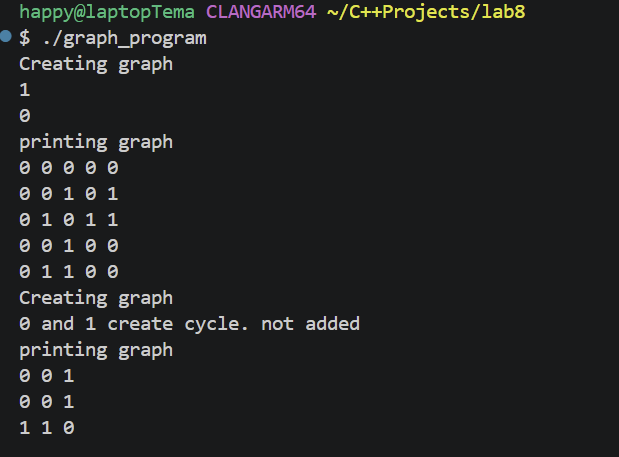
\includegraphics[width=0.85\textwidth]{lab8_1}
    \captionsetup{justification=centering}
    \captionof{figure}{Результат работы программы}
\end{center}

\section{Вывод}
В данной лабораторной работе были получен навык разработки шаблонов классов
\end{document}